\documentclass[11pt,a4paper]{article}
\usepackage[margin=2.5cm]{geometry}
\usepackage[utf8]{inputenc}
\usepackage[T1]{fontenc}
\usepackage{hyperref}
\renewcommand{\familydefault}{\sfdefault}
\usepackage{helvet}
\pagestyle{empty}
\usepackage[kerning=true]{microtype}
\usepackage{parskip}
\usepackage{sansmath}
\usepackage[font={small, bf}]{caption}
\usepackage[font={small}]{subcaption}
\usepackage{graphicx}
\usepackage{multicol}
\setlength{\abovecaptionskip}{0pt}
\setlength{\floatsep}{10pt}
\setlength{\textfloatsep}{0pt}
\setlength{\intextsep}{0pt}
\setlength{\belowcaptionskip}{0pt}
\setlength{\parindent}{5ex}
\setlength{\parskip}{0pt}
% Feel free to use additional packages for glosses, figures, whatnot.

% The next bit is for reserving sufficient space for authors,
% affiliations, and e-mail address.  No need to change for initial
% anonymous version.  For the final version, replace the
% \toggletrue{anonymous} with \togglefalse{anonymous} to de-anonymize.
\usepackage{etoolbox}
\newtoggle{anonymous}
\togglefalse{anonymous}

\renewcommand{\title}[1]{\textbf{#1}\\}
\newcommand{\authors}[1]{\iftoggle{anonymous}{\phantom{#1}}{#1}\\}
\newcommand{\email}[1]{\iftoggle{anonymous}{\phantom{#1}}{#1}}

\begin{document}

% First page:

% Insert title, authors, affiliations, and e-mail address in the next three lines:
\noindent\title{4-5 year old children can successfully communicate using ad-hoc referential expressions}
\authors{Veronica Boyce, Ilaria Chen, Bobby Sparks, Malia Perez, Michael C. Frank} 
\email{vboyce@stanford.edu;  Stanford University}
\newline
%

% Intro
%TODO citations

%TODO math

%TODO crossref figures!

As children acquire language, they must master many communication skills such as using metaphor and tracking the knowledge state of their partner. Adults demonstrate these communicative abilities in iterated reference games, where they describe novel figures to partners with high accuracy. Over repetitions, description length reduces as pairs come to share nicknames for the figures (Clark \& Wilkes-Gibbs 1986, Hawkins et al. 2020). This paradigm is commonly used with adults, but the consensus has been that tracking ad-hoc references in this way is too difficult for young children (in part due to notable failures in the literature; Glucksberg et al., 1966). We revisit this question, using a simplified method adapted from Leung et al. 2020.

\bigskip
\textbf{Methods:} Pairs of children played a matching game on tablets. On each trial, the ``speaker'' child would see two images, one in a box, and describe the boxed image (orally) to their partner (Fig 1). The ``listener'' child saw the same two images and was tasked with helping Smurfy (a stuffy) guess the matching target image by touching it on the screen. Children alternated roles trial by trial; the children passed Smurfy back and forth to track their roles. The 4 target images were a subset of stimuli from Leung et al. 2020; distractors were drawn from the set of other targets. Children completed 2 practice trials with familiar shapes, and then 12 target trials (3 blocks of the 4 target images; Fig 1). We recruited 4-5 year old children from a university preschool; 20 pairs completed at least 8 out of 12 target trials and were included in the analysis. Utterances were transcribed from video recording using Whisper and then hand-checked. 
% Results

\bigskip

\textbf{Results:} 
Children uses a variety of different referential expressions to successfully convey the target to their partner (see Examples on next page). Children were 84\% accurate at selecting the target image, and accuracy was relatively stable over time ($\beta=$0.13 [-.04, .31]; Fig 2A). Children's speed to select a target increased over time ($\beta=$-1.24 [-1.89, -.59]; Fig 2B). Children generally produced short descriptions, and the length of descriptions tended to slightly increase over time ($\beta=$0.11 [-.03, .25]; Fig 2C). 

To compare the similarities of children's descriptions to those of their partners and other children, we embedded the utterances using S-BERT (Reimers \& Gurevych 2019) and used pairwise cosine similarity of embeddings as a proxy for utterance similarity. Children's utterances for an image are most similar to their own descriptions of the same image in different blocks (Fig 3). However, children's descriptions for an image are more similar to their partner's descriptions than the descriptions of children in other games. This indicates some level of partner specificity: children are not just talking past each other but are influenced by their partners prior descriptions.

\bigskip

\textbf{Caveats and Future Directions:} 
Transcripts of the sessions revealed that the research assistant echoed the children's descriptions on the majority of trials (ex: ``Mary says she sees a bear. Do you see a bear?''). While this did not introduce any new descriptions, the repetition could potentially lend ``authority'' to the description and influence children. Additionally, we have a limited sample of only 20 pairs of children, 4 images, and 3 repetitions. In a planned experiment 2, we will replicate this experiment, with a clearer experimenter script to avoid echoing and additional tweaks to clarify the procedure. 

This preliminary study suggests that (contra Glucksberg et al.) 4-5 year old children \textbf{can} describe and select novel figures with each other at above chance accuracy. However, the initially short utterances and lack of reduction offers intriguing suggestions about possible differences between children's and adult's approaches to to iterated reference games. These could be due to different linguistic abilities, social expectations, or differential task difficulty. 
\newpage

\begin{figure}
%TODO open materials
	\caption{Schematic of methods}
 \begin{center}{ 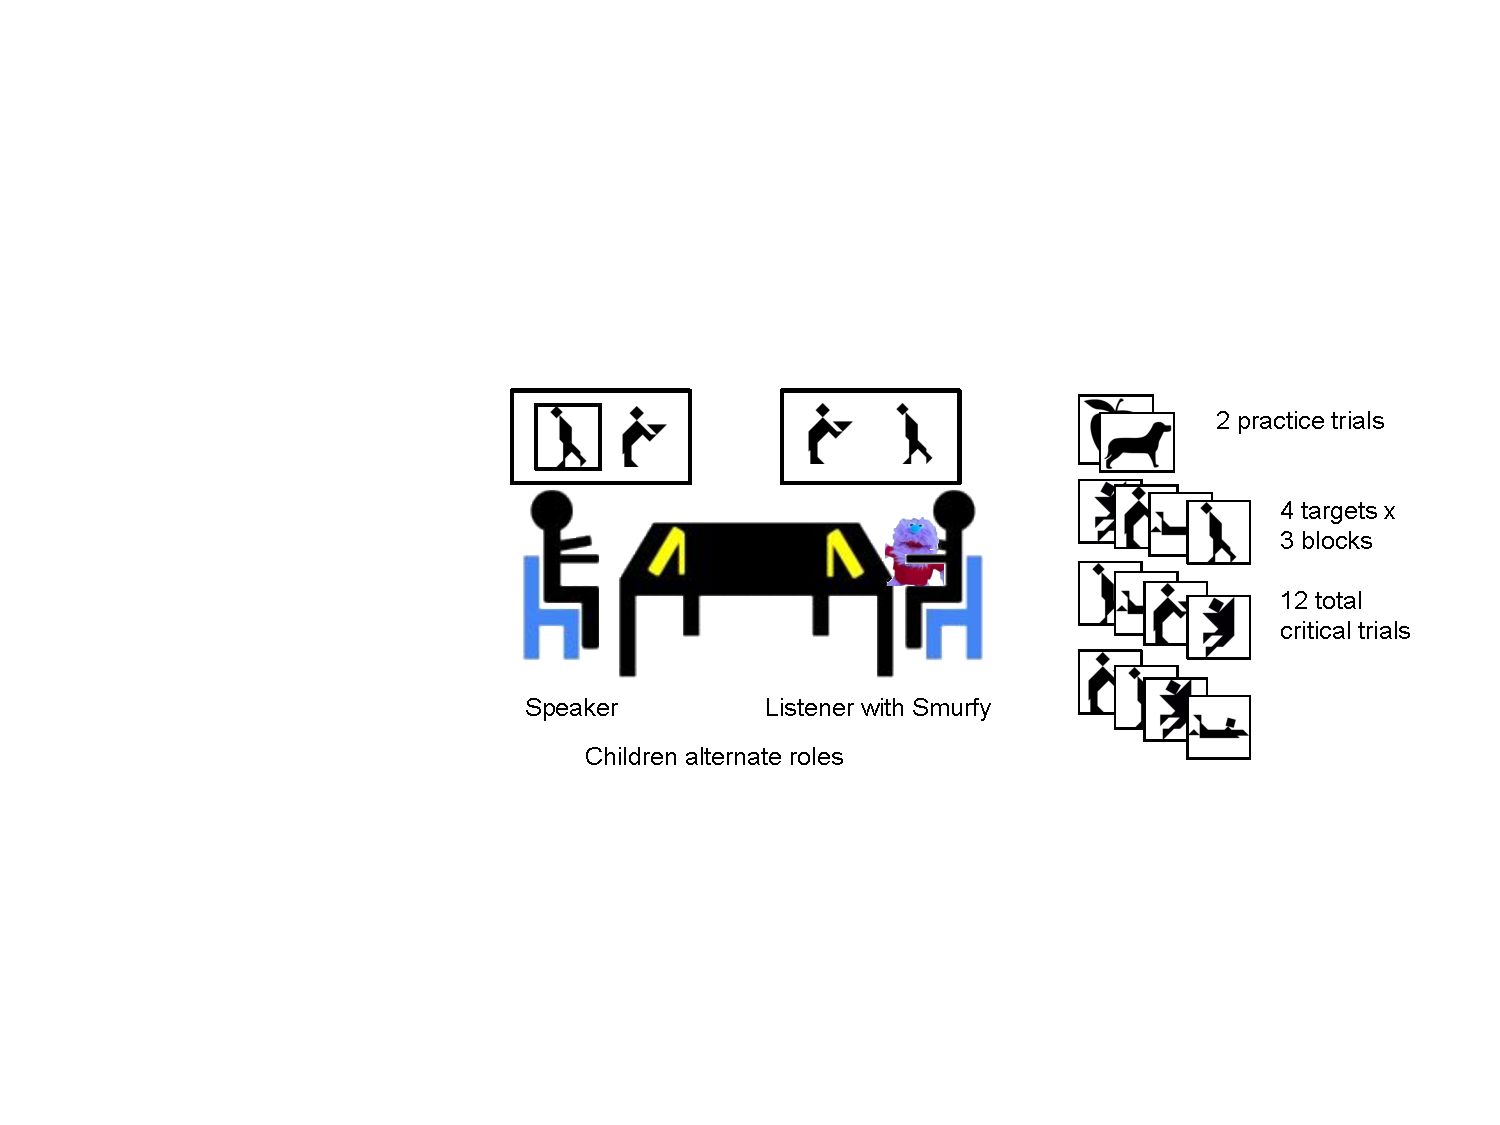
\includegraphics[width=.8\textwidth, trim={8cm 6cm 1cm 6.4cm}, clip]{exp-diagram.pdf}}
 	\end{center}
 	\begin{small}
 	20 pairs of children played a matching game on tablets while facing each other across a table. Each game consisted of 2 practice trials and 12 critical trials. 
 	\end{small}

\end{figure}
	\begin{figure}
		\begin{minipage}{.5\textwidth}
			\captionof{figure}{Results}
			{	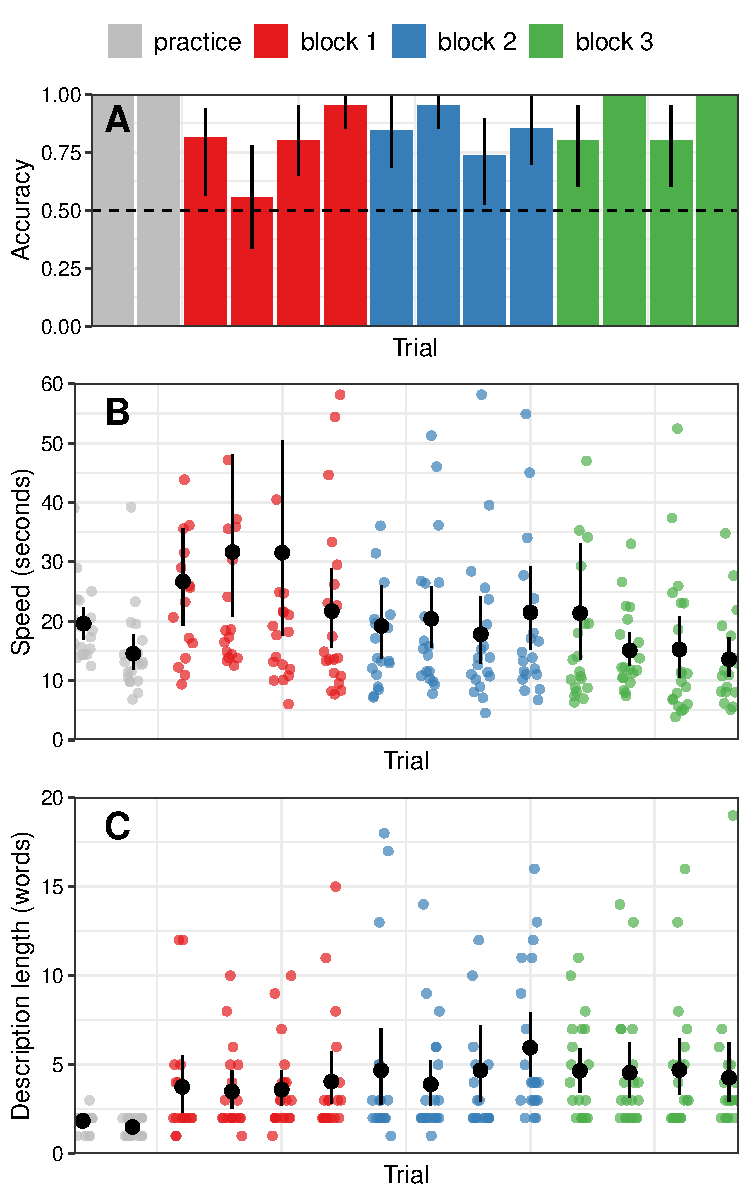
\includegraphics[width=\textwidth]{plot1.pdf}} 
			\begin{small}
			\textbf{	A.} Children's accuracy is at ceiling on practice trials and above chance on target trials.\textbf{ B.} Children speed up over time on target trials. \textbf{C.} Children's descriptions are usually short, but do not reduce in length over time. 
				
			\end{small}
			
		\end{minipage}
		~~~
		\begin{minipage}{.5\textwidth}	
		\captionof{figure}{Similarity Results}
		{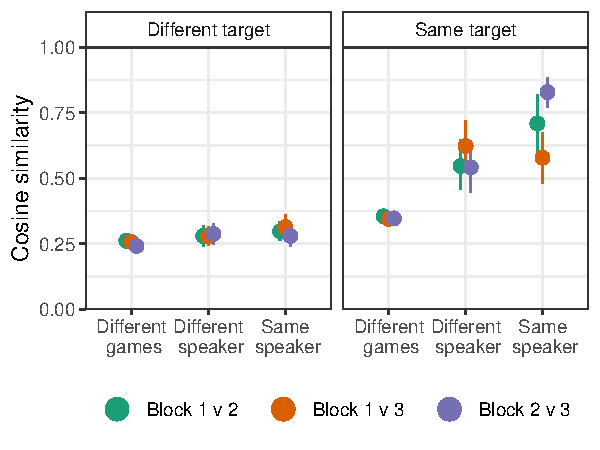
\includegraphics[width=\textwidth]{sims.pdf}} 
		\begin{small}
		Descriptions given by children were compared using sentence embeddings. Descriptions were most similar when provided by the same child for the same image. However, children described images more similarly to their partners than to children in other games.  Across games, the same image is described more similarly than different images.
		\end{small}
		
		\bigskip
		\begin{small}
\textbf{\centering Example successful descriptions:\\}
\smallskip
		a person $\bullet$ a person walking $\bullet$ sad walking $\bullet$ a man with two foot and a diamond shaped tummy and a square head
		
		\smallskip
		a flying person $\bullet$
		a superhero$\bullet$
		somebody jumping $\bullet$ two wings with a square in the back with two feet
		\smallskip
		
		someone building a funnel $\bullet$
		a server$\bullet$
		a person holding up a plate $\bullet$ a man with one foot and a line and a square and a triangle
		\smallskip
		
		a crocodile tasting an animal in the water$\bullet$
		a whale$\bullet$
		someone flying a plane without a cover$\bullet$
		a person lying on the ground
		
		\end{small}
		\end{minipage}
	\end{figure}



\begin{figure}
	\begin{small} \textbf{References:}
Leung, Hawkins, Yurovsky. Cogsci, 2020. $\bullet$ Glucksberg, Krauss, Weisberg. J of Expt Child Psychology, 1966. $\bullet$ Clark \& Wilkes-Gibbs. Cognition, 1986. $\bullet$ Hawkins, Frank, Goodman. Cognitive Science, 2020. $\bullet$ Reimers \& Gurevych. arXiv 2019.
\end{small}
\end{figure}
\end{document}